\documentclass[a4paper]{article}

\usepackage[pages=all, color=black, position={current page.south}, placement=bottom, scale=1, opacity=1, vshift=5mm]{background}
\SetBgContents{
	\tt This work is shared under a \href{https://creativecommons.org/licenses/by-sa/4.0/}{CC BY-SA 4.0 license} unless otherwise noted
}      % copyright

\usepackage[margin=1in]{geometry} % full-width

% AMS Packages
\usepackage{amsmath}
\usepackage{amsthm}
\usepackage{amssymb}
\usepackage{babel}
% Unicode
\usepackage[utf8]{inputenc}
\usepackage{hyperref}
\hypersetup{
	unicode,
%	colorlinks,
%	breaklinks,
%	urlcolor=cyan, 
%	linkcolor=blue, 
	pdfauthor={Author One, Author Two, Author Three},
	pdftitle={A simple article template},
	pdfsubject={A simple article template},
	pdfkeywords={article, template, simple},
	pdfproducer={LaTeX},
	pdfcreator={pdflatex}
}

% Vietnamese
%\usepackage{vntex}

% Natbib
\usepackage[sort&compress,numbers,square]{natbib}
\bibliographystyle{mplainnat}

% Theorem, Lemma, etc
\theoremstyle{plain}
\newtheorem{theorem}{Theorem}
\newtheorem{corollary}[theorem]{Corollary}
\newtheorem{lemma}[theorem]{Lemma}
\newtheorem{claim}{Claim}[theorem]
\newtheorem{axiom}[theorem]{Axiom}
\newtheorem{conjecture}[theorem]{Conjecture}
\newtheorem{fact}[theorem]{Fact}
\newtheorem{hypothesis}[theorem]{Hypothesis}
\newtheorem{assumption}[theorem]{Assumption}
\newtheorem{proposition}[theorem]{Proposition}
\newtheorem{criterion}[theorem]{Criterion}
\theoremstyle{definition}
\newtheorem{definition}[theorem]{Definition}
\newtheorem{example}[theorem]{Example}
\newtheorem{remark}[theorem]{Remark}
\newtheorem{problem}[theorem]{Problem}
\newtheorem{principle}[theorem]{Principle}

\usepackage{graphicx, color}
\graphicspath{{fig/}}

%\usepackage[linesnumbered,ruled,vlined,commentsnumbered]{algorithm2e} % use algorithm2e for typesetting algorithms
\usepackage{algorithm, algpseudocode} % use algorithm and algorithmicx for typesetting algorithms
\usepackage{mathrsfs} % for \mathscr command

\usepackage{lipsum}

% Author info
\title{Longitudinal analysis of Disturbed dynamo magnetic signatures}
\author{Castellanos-Velazco C. I.$^{1,3}$ \and Corona-Romero P.$^{2,3}$ \and Sergeeva M.$^{2,3}$}

\date{
	$^1$Universidad Nacional Autonoma de Mexico, Posgrado en Ciencias de la Tierra \\ %\texttt{\{auth1, auth3\}@org1.edu}\\%
	$^2$ Laboratorio Nacional de Clima Espacial \\
	$^3$ Instituto de Geofisica
	% \texttt{auth3@inst2.edu}\\[2ex]%
%	\today
}

\begin{document}
	\maketitle
	
	\begin{abstract}
		
		The present study seeks to analyze longitudinally, the magnetic fluctuations associated with the disturbed dynamo electric field (DDEF) using 11 observatories encircling the globe at mid-low latitudes. The event to be studied is the geomagnetic storm known as the Saint Patrick event due to his main phase was developing during that celebration (march 17th, 2015).In the present studio, we perform a wavelet spectrum in combination with cross-wavelet technique and a semblance analysis studio in order to isolate the DDEF magnetic signatures.  
		\\
		
		\noindent\textbf{Keywords:} Disturbed dynamo, wavelet
	\end{abstract}

	\tableofcontents
	
	\section{Introduction}
	\label{sec:intro}
		
	During geomagnetic storms (GS), one of the responses which arise in the ionosphere is the driving of electric currents. In the case of mid-low geomagnetic latitude ranges, we highlight the presence of the Disturbed dynamo (Ddyn) and the disturbed polar current number 2 (DP2). \\
	
	\subsection{Geomagnetic Data}
	The geomagnetic data analyzed in this paper corresponded to the observatories shown within the Table \ref{tab:obs}. magnetic data can be obtained from INTERMAGNET (\textit{International Real-Time Magnetic Observatory Network} \citep{intermagnet})  where as it is shown, all the observatories are present within the a narrow range of magnetic latitude ($21 - 33^\circ$). On the other hand, this observatories envelope quite different Universal Time (UT) zones. We have to deal with limitations for the aim of this project due to the lack of data availability for some observatories during the period of interest combined with the absence of observatories at some points. In the end it was decided to divide the longitudinal study in five sectors in function of the UT zones for each observatory:
	
	\begin{enumerate}
		\item sector 1: GUI (UTC 0), TAM (UTC 1) 
		\item sector 2: JAI (UTC 5:30)
		\item sector 3: LZH, BMT (UTC 8), CYG, KNY, KAK (UTC 9)
		\item sector 4: HON (UTC -10)
		\item sector 5: TEO (UTC -6), SJG (UTC -4) 
	\end{enumerate}
	
	Although the distance between each observatory presents a limitation for studying the longitudinal develop of the GS, we can still analyze the response for different time sectors in which each observatory was present during the main phase. 
	
\begin{table}[htbp]
	\caption{List of observatories considered for this study.}
	\begin{tabular}{lccccccc}
		\hline
		Country & \multicolumn{1}{l}{Observatory} & \multicolumn{1}{l}{IAGA code} & \multicolumn{1}{l}{geographic } & \multicolumn{1}{l}{geographyc } & \multicolumn{1}{l}{magnetic} & \multicolumn{1}{l}{magnetic } & \multicolumn{1}{l}{UT} \\ 
		& \multicolumn{1}{l}{} & \multicolumn{1}{l}{} & \multicolumn{1}{l}{latitude} & \multicolumn{1}{l}{longitude} & \multicolumn{1}{l}{latitude} & \multicolumn{1}{l}{longitude} & \multicolumn{1}{l}{h} \\ \hline
		China & Beijing & BMT & 40.3 N & 116.2 E & 30.53 N & 172 W & 8 \\ 
		South Korea & Cheongyang & CYG & 36.37 N & 126.854 E & 27 N & 162.43 W & 9 \\ 
		India & Jaipur & JAI & 26.917 N & 75.8 E & 18.42 N & 150.47 E & 5.5 \\ 
		Spain & Guimar & GUI & 28.317 N & 16.433 W & 33.21 N & 61.1 E & 0 \\ 
		USA & Honolulu & HON & 21.317 N & 158 W & 21.49 N & 90.03 W & -10 \\ 
		Japan & Kakioka & KAK & 36.232 N & 140.186 E & 27.8 N & 149.73 W & 8 \\ 
		Japan & Kanoya & KNY & 31.417 N & 130.867 W & 22.3 N & 158.4 W & 9 \\ 
		China & Lanzhou & LZH & 36.083 N & 103.833 E & 26.23 N & 176.79 E & 8 \\ 
		USA, Puerto Rico & San Juan & SJG & 18.11 N & 66.15 W & 28.19 N & 6.1 E & -4 \\ 
		Argelia & Tamanraset & TAM & 22.783 N & 5.571 E & 24.3 N & 82.29 E & 1 \\
		Mexico & Teoloyucan & TEO & 19.747 N & 99.182 W & 27.81 N & 28.4 W & -6 \\  \hline
	\end{tabular}
	\label{tab:obs}
\end{table}


\begin{figure}
	\centering
	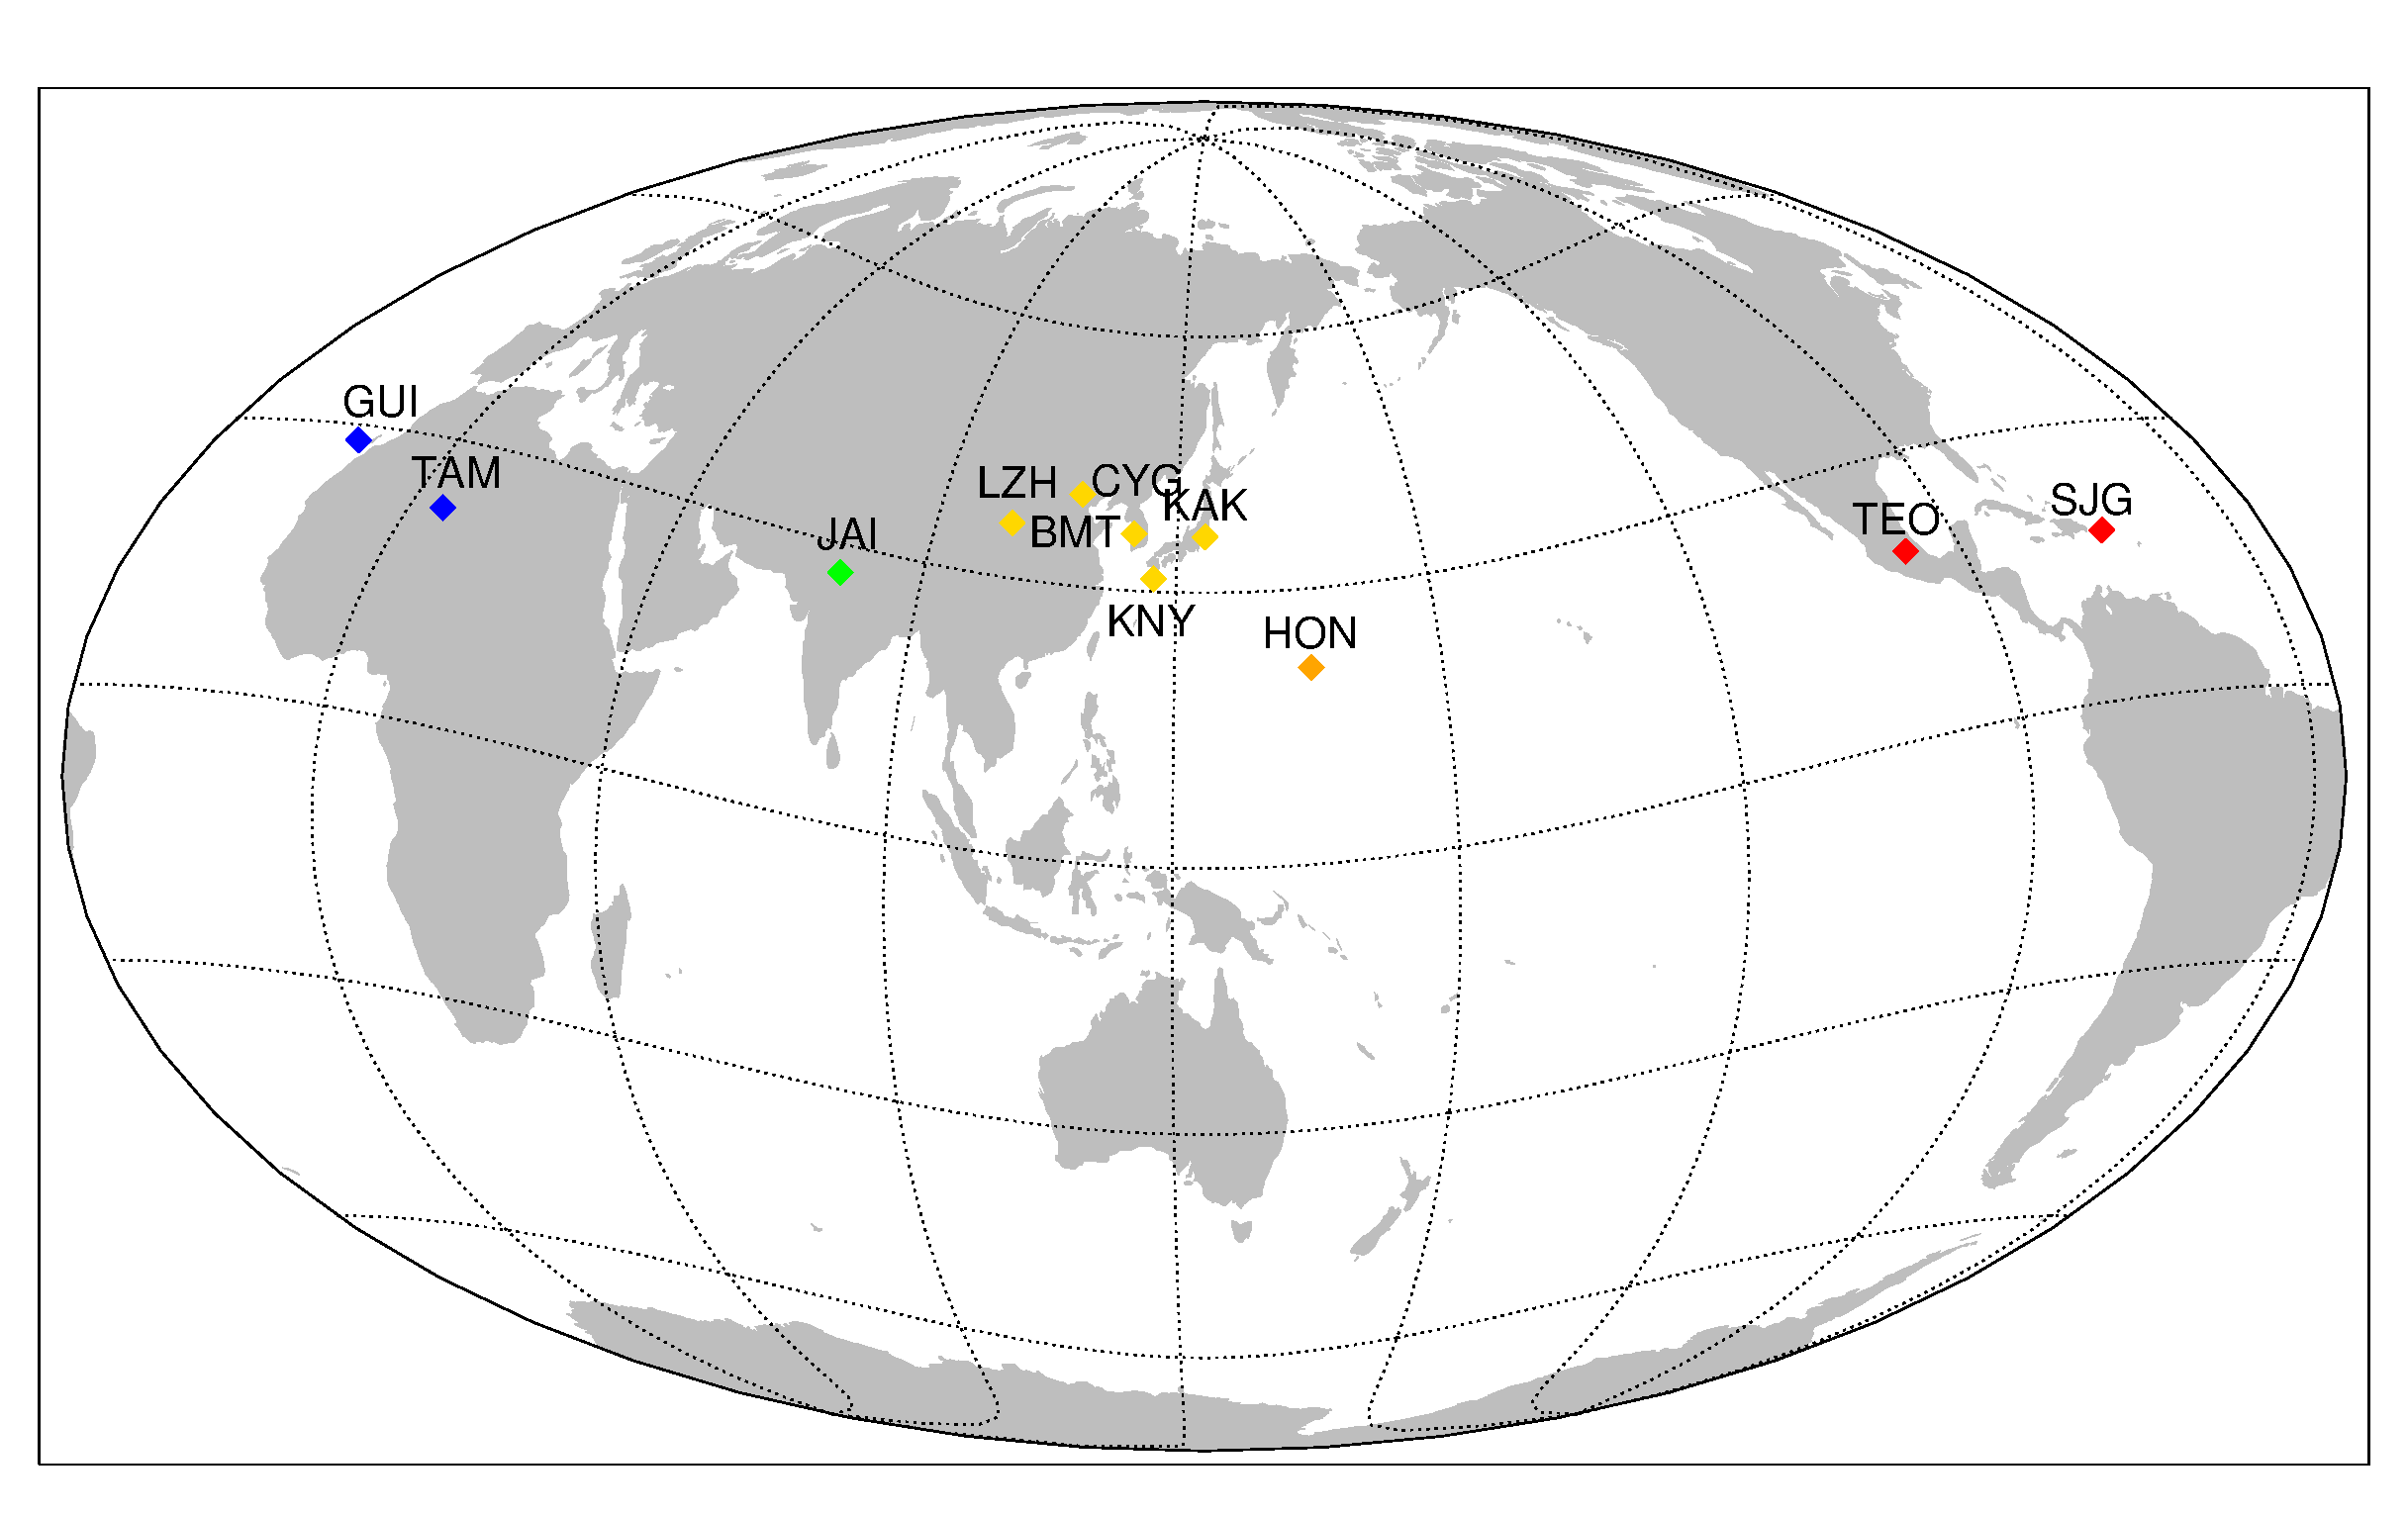
\includegraphics[width=0.7\textwidth]{fig/map.eps}
	\caption{Geographic position of every magnetic observatory considered for this study. The color code corresponds to different local time regions: blue (UT 0, 1), green (UT 5:30), yellow (UT 8, 9), orange (UT -10), red (-6, -4).}
	\label{fig:map}
\end{figure}


	\section{Methodology}
	\label{sec:method}
	\subsection{Processing magnetic data}
	
	\subsection{Isolation of magnetic fluctuations of ionospheric origin}
	According to \cite{1969intro_to_iono_p, l_handbook_geof_sw_Geom_field, baseline_Gjerloev, vanKampt}, we can approach the recordings of a local magnetometer as:
	\begin{equation}
		H_{loc} = H_{SQ} + H_0 + H_{MT} + H_{I},
	\end{equation}
	\noindent where $H_{SQ}$ is the diurnal variation and $H_0$ is the monthly baseline. $H_{MT}$ on the other hand are the variations induced due to the magnetospheric currents activity and intensification during GS. Finally, $H_I$ stands for the magnetic variations driven by ionospheric currents activity during a GS.\\
	
	For mid-low magnetic latitudes, we can approach roughly enough $H_{MT}$ as $H_{MT} \approx SYM - H \cdot cos(\lambda)$, being $\lambda$ the geomagnetic latitude of certain observatory. Thus $H_I$ can be approached by:
	
	\begin{equation}
		H_I = H_{DDEF} + H_{PPEF} \approx H_{loc} - (H_{SQ} + H_0 + SYM-H \cdot cos(\lambda))
	\end{equation}
	
	\noindent being $H_{DDEF}$ and $H_{PPEF}$ the magnetic field associated with the disturbed dynamo electric fields and the prompt penetration electric fields respectively.\\
	
	
	\subsection{Time-Frequency Analysis}
	In order to isolate $H_{DDEF}$ and $H_{PPEF}$ from each other, we can proceed from the consideration that both ionospheric currents induce quasi periodic fluctuation \cite{nishida_68_fluctuations, blanc_ddyn, amory2020_filtros}. Hence we begin with a Fourier Analysis, setting passband filters for fluctuations of periods ~24 h to reconstruct $H_{DDEF}$, meanwhile using highpass filters to reconstruct $H_{PPEF}$.\\
	
	However, from \cite{CASTELLANOSVELAZCO2024} it is concluded the need of compliment the analysis, performing wavelet techniques \cite{APracticalGuidetoWaveletAnalysis}, as shown in \cite{amory_younas2021} where they performed a crosswavelet transform to $H_{SQ}$ and $H_I$. Thus, they applied a semblance analysis \cite{cooper_semblance}. The purpose of such process is to compare to time series ($H_{SQ}$ and $H_I$) which have similar band frequency fluctuations ($f \approx 1.15e-5 Hz$ or $T \approx 24 h$) identify which signal is more correlated to $H_{DDEF}$ activity.\\
	
	
	For the present paper, we performed a wavelet analysis ($W$), using the Morlet function as mother wavelet. Hence we computed the wavelet spectrum ($|\psi_0|^2$) in order to observe the power of the signal related to $H_I$. As second stage of this time-frequency analysis, we computed the cross-wavelet:
	
	\begin{equation}
		\label{eq:xwt}
		W_n^{SQ,H_I}(s) = W_n^{H_{SQ}}(s) W_n^{H_I *}(s),
	\end{equation}
	\noindent being $s$ the scale of the wavelet transform, $n$ the index number of each time series. In the right side of equation \ref{eq:xwt} $W_n^{H_{SQ}}(s)$ is the wavelet transform applied to the diurnal variation meanwhile $ W_n^{H_I *}(s)$ is the conjugate of the wavelet transform applied to $H_I$. The output of this crosswavelet transform we are interested in, are the resulting amplitude $\alpha$ and the local phase $\theta$. Hence we carry out a semblance analysis described by the following equation:
	
	\begin{equation}
		semblance = cos ^n(\theta)
	\end{equation}
	
	\noindent being $n$ an odd integer number greater than 1. For this work we decided to set $n=9$ as tested in \cite{cooper_semblance}. From semblance we can obtain a normalized correlation values ranging between -1 and 1, where values closer to -1 are highly correlated to $H_I$, meanwhile values closer to 1 are more correlated to $H_{SQ}$. however, considering that semblance does not give information about the intensity of neither of the implied signals, we can multiply it by the amplitude $\alpha$ and compute $H_{DDEF}$ likewise:
	
	\begin{equation}
		H_{DDEF} = \alpha \cdot anticorr(semblance),
	\end{equation}
	\noindent since we are not interested in those signals correlated to $H_{SQ}$. Having the wavelet spectrum $|\psi_0(n)|^2$ which give us the power of the signals and $\alpha \cdot anticorr(semblance)$ which highlights the signal related to $H_{DDEF}$, we can observe not only weather $H_{DDEF}$ variations are present during the event but also, their intensity. 
	
	\section{Results}
	\label{sec:prev-results}
	\subsection{Fourier Analysis}

	\subsection{Wavelet Analysis}
	
	\section{Discussion}
	
	\section{conclusions}
	
	The Ddyn magnetic fluctuations, $H_{DDEF}$ where present in TEO observatory with more intensity since []\\
	
	Another observation found is that TEO is the point at which we observe picks of $H_{PPEF}$ significantly higher than $H_{DDEF}$ fluctuations, but is also the point at which $H_{PPEF}$ gets highest values during this study,\\
	
	On the other hand, in the results obtained through analyzing magnetic data from observatories within sector 3 which corresponds to LZH, BMT, CYG, KNY and KAK we observe very weak and even null $H_{DDEF}$. This is consistent with [...].\\
	
	
	\paragraph{Acknowledgements} \lipsum[6]
	
%	\newpage
	\bibliography{ref_longstudio}
	
	\appendix
	

	
\end{document}